\documentclass[10pt]{beamer}
\usepackage{amsmath,amssymb,longtable,hhline}
\usepackage{mathrsfs}
\usepackage{xcolor}
\usepackage{listings}
\usepackage{hyperref}
\usepackage{multicol}
\usepackage{anyfontsize}
\usepackage{minted}

\usemintedstyle{tango}
\newcommand{\ltprgsize}{\fontsize{5}{5}\selectfont}
\setminted{fontsize=\ltprgsize,mathescape}

\definecolor{mygreen}{rgb}{0,0.6,0}
\definecolor{mygray}{rgb}{0.5,0.5,0.5}
\definecolor{mymauve}{rgb}{0.58,0,0.82}

\hypersetup{
    bookmarks=true,         % show bookmarks bar?
    unicode=true,           % non-Latin characters in Acrobat’s bookmarks
    pdftoolbar=false,        % show Acrobat’s toolbar?
    pdfmenubar=false,        % show Acrobat’s menu?
    pdffitwindow=false,     % window fit to page when opened
    pdfstartview={FitH},    % fits the width of the page to the window
    pdftitle={Компьютерная алгебра в задачах оптимизации},    % title
    pdfauthor={Evgeny Cherkashin, Seseg Badmatsyrenova},     % author
    pdfsubject={symbolic computations},   % subject of the document
    pdfnewwindow=true,      % links in new PDF window
    colorlinks=true,       % false: boxed links; true: colored links
    linkcolor=red,          % color of internal links (change box color with linkbordercolor)
    citecolor=green,        % color of links to bibliography
    filecolor=magenta,      % color of file links
    urlcolor=blue           % color of external links
}

\lstset{language=Python,
  basicstyle=\footnotesize\ttfamily,        % the size of the fonts that are used for the code
  breakatwhitespace=false,         % sets if automatic breaks should only happen at whitespace
  breaklines=true,                 % sets automatic line breaking
  captionpos=b,                    % sets the caption-position to bottom
  commentstyle=\color{mygreen},    % comment style
  escapeinside={\%*}{*)},          % if you want to add LaTeX within your code
  extendedchars=true,              % lets you use non-ASCII characters; for 8-bits encodings only, does not work with UTF-8
%  frame=single,                    % adds a frame around the code
  keepspaces=true,                 % keeps spaces in text, useful for keeping indentation of code (possibly needs columns=flexible)
  keywordstyle=\color{blue},       % keyword style
%  numbers=left,                    % where to put the line-numbers; possible values are (none, left, right)
  numbersep=5pt,                   % how far the line-numbers are from the code
  numberstyle=\tiny\color{mygray}, % the style that is used for the line-numbers
  rulecolor=\color{black},         % if not set, the frame-color may be changed on line-breaks within not-black text (e.g. comments (green here))
  showspaces=false,                % show spaces everywhere adding particular underscores; it overrides 'showstringspaces'
  showstringspaces=false,          % underline spaces within strings only
  showtabs=false,                  % show tabs within strings adding particular underscores
  stepnumber=2,                    % the step between two line-numbers. If it's 1, each line will be numbered
  stringstyle=\color{mymauve},     % string literal style
  tabsize=2,                       % sets default tabsize to 2 spaces
%  title=\lstname                   % show the filename of files included with \lstinputlisting; also try caption instead of
}
\usepackage{pifont}

\usetheme{Warsaw}
\usecolortheme{crane}
%\useinnertheme{rectangles}
\setbeamertemplate{itemize item}{\scriptsize\hbox{\donotcoloroutermaths\ding{113}}}
\setbeamertemplate{itemize subitem}{\tiny\raise1.5pt\hbox{\donotcoloroutermaths$\blacktriangleright$}}
\setbeamertemplate{itemize subsubitem}{\tiny\raise1.5pt\hbox{\donotcoloroutermaths$\blacktriangleright$}}
\setbeamertemplate{enumerate item}{\insertenumlabel.}
\setbeamertemplate{enumerate subitem}{\insertenumlabel.\insertsubenumlabel}
\setbeamertemplate{enumerate subsubitem}{\insertenumlabel.\insertsubenumlabel.\insertsubsubenumlabel}
\setbeamertemplate{enumerate mini template}{\insertenumlabel}

\beamertemplatenavigationsymbolsempty

\usepackage{iftex,ifxetex}
\ifPDFTeX
  \usepackage[utf8]{inputenc}
  \usepackage[T1]{fontenc}
  \usepackage[russian]{babel}
  \usepackage{lmodern}
  \usefonttheme{serif}
\else
  \ifluatex
    \usepackage{unicode-math}
    \defaultfontfeatures{Ligatures=TeX,Numbers=OldStyle}
    \setmathfont{Latin Modern Math}
    \setsansfont{Linux Biolinum O}
    \setmonofont{Fira Mono}
    \usefonttheme{professionalfonts}
    % \setmathfont[
    %     Ligatures=TeX,
    %     Scale=MatchLowercase,
    %     math-style=upright,
    %     vargreek-shape=unicode
    %     ]{euler.otf}
  \fi
\fi

%\useoutertheme{split}
%\useinnertheme{rounded}
\setbeamertemplate{background canvas}[vertical shading][bottom=white!80!cyan!20,top=cyan!10]
%\setbeamertemplate{sidebar canvas left}[horizontal shading][left=white!40!black,right=black]

\graphicspath{{pics/}}

\providecommand{\email}[1]{\texttt{#1}}

% --------------------------

\begin{document}
\title[Model Driven Architecture Implementation using Linked Data]{Model Driven Architecture Implementation using Linked Data}
\author[E.~Cherkashin, A.~Kopaygorodsky, L.~Kazi, A.~Shigarov, V.~Paramonov]{\bfseries%
  Evgeny Cherkashin, Alexey Kopaygorodsky, Ljubica Kazi, Alexey Shigarov, Vyacheslav Paramonov}
\institute[ISDCT SB RAS, ESI SB RAS, ISC SB RAS, University of Novi Sad, Technical faculty "Mihajlo Pupin",
National Research Irkutsk State Technical University]{\normalsize ISDCT SB RAS, ESI SB RAS, ISC SB RAS, National Research Irkutsk State Technical University, Irkutsk,Russia,\\
  University of Novi Sad, Technical faculty "Mihajlo Pupin", Zrenjanin, Serbia\\[1em]
\email{\href{mailto:eugeneai@icc.ru}{eugeneai@icc.ru},\href{mailto:digger@istu.edu}{digger@istu.edu}}%
}
\date[2018]{{}\\
The 24${}^\text{th}$ International Conference on Information\\ and Software Technologies (ICIST 2018)\\
October 4${}^\text{th}$ -- 6${}^\text{th}$, 2018\\
Vilnius, Lithuania
}
%\date{\today}
\maketitle
\begin{frame}
  \frametitle{Research objectives}
  \textbf{Main objective} of the research is to construct a MDA technology based on nowadays system modeling visual languages (SysML,BPMN,CMMN) and existing Semantic Web \textbf{vocabularies}. The following techniques and software are under development:
  \begin{enumerate}
  \item CIM representation with SysML, BPMN, CMMN, and results of source code processing,
  \item CIM, PIM, PSM representation in RDF with existing vocabularies,
  \item transformation implementation with logical language Logtalk,
  \item usage of LOD sources in the transformations,
  \item generation of documents and interfaces with LOD markup.
  \end{enumerate}
\end{frame}
\begin{frame}
  \frametitle{Model Driven Architecture and Linked Open Data}
  \begin{center}
    \includegraphics[width=0.9\linewidth]{mda-overview.pdf}
  \end{center}
\end{frame}
\begin{frame}
  \frametitle{MDA component architecture}
  \centering
  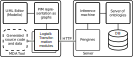
\includegraphics[width=1\linewidth]{architecture-mda-lod-ext.pdf}
\end{frame}
\begin{frame}
  \frametitle{Logtalk as transformation definition language}
  We have chosen Logtalk as it
  \begin{itemize}
  \item inherits widely known Prolog language syntax and runtime;
  \item implemented as macro package, performance penalties are about 1.5\%;
  \item has flexible semantics: we can define transformations and constraints within the same syntax;
  \item implement object-oriented knowledge (rules) structuring, encapsulation and replacement;
  \item compositional way of transformation implementation;
  \item powerful engine to post constraints on object-to-object messages (events);
  \item has implementation for many Prolog engines.
  \end{itemize}
  The <<regular>> language allow us to use its libraries not directly related to MDA transformations.
\end{frame}
\begin{frame}[fragile]
  \frametitle{Semantic Web technologies in representation of models
    during transformation}
  \begin{itemize}
  \item Assimilates experience of domain basic researches trending to standardization;
  \item regular set of triples denote a graph (T-Box, A-Box);
  \item standard vocabularies are formally described (\verb|rdfs:range|,\verb|rdfs:domain|);
  \item supported with most programming systems (libraries, inference engines, SPARQL);
  \item has a way of global element identification;
  \item SWI-Prolog supports direct queries to a graph, as well as interpreting some predicates (\verb|dc:title|, \verb|rdfs:label|), encapsulating sparse RDF structure into a predicate arguments;
  \item there is simple way of data security implementation (\verb|rdfs:seeAlso|);
  \item by means of Semantic Web \& LOD we are able to encapsulate data transmission between heterogeneous information systems;
  \end{itemize}
\end{frame}


\begin{frame}
  \frametitle{Architecture of transformation modules}
  \centering
  \includegraphics[width=0.9\linewidth]{architect_tree_pres-en-wo-OCL.pdf}
\end{frame}

\begin{frame}[fragile]
  \frametitle{PSM: Class structure inference}

%\begin{multicols}{2}
\begin{minted}{logtalk}
:- object(direct(_Package,_LocalProf,_CodeProf)).    % Transformation driver object
:- public([tr/4,tr/3]).                              % Public interface of a class synthesis scenario
:- protected([package/1, profiles/2, profile/1]).
package(Package):- parameter(1, Package).            % Access to the parameter of the object
profile(Profile):- parameter(2, Profile).
profile(Profile):- parameter(3, Profile).
profiles(L):-
    findall(Profile, ::profile(Profile), L).
tr(class, Class, ClassID):- ::package(Package),      % Synthesize a class
    query(Package)::class(Name, ClassID),            % Query package structure in XMI
    create_object(Class,                             % Create a <<Class>> object
        [instantiates(class)],[],[]),
    create_object(Attributes,                        % Create <<Attributes>> object
        [instantiates(params)],[],[]),
    create_object(Methods,                           % ...<<Methods>>.
        [instantiates(methodlist)],[],[]),
    Class::name(Name),                               % Name the class.
    forall(                                          % Generate attributes of the class,
        ::tr(attribute,Attribute,ClassID,_AttrID),   % organizing them in a local database.
        Attributes::append(Attribute) ),
    forall(                                          % ...methods...
        ::tr(method, Method, ClassID, _MethodID),
        Methods::append(Method) ),
    Class::attributes(Attributes),                   % Set the attributes for the class.
    Class::methods(Methods).                         % ...methods.
tr(attribute, Attribute, ClassID, AttributeID):-     % Attribute transformations
    ::package(Package),
    query(Package)::attribute(Name,ClassID,AttrID),
    create_object(Attribute,
        [instantiates(param)],[],[]),
    Attribute::name(Name).                           % Name the attribute.
tr(method, Method, ClassID, MethodID):-              % Transformation of methods
    ::package(Package),
    query(Package)::method(Name,ClassID,MethodID),
    create_object(Method,
    [instantiates(method)],[],[]),
    Method::name(Name).                              % Name of the method
:- end_object.
\end{minted}
%\end{multicols}
\end{frame}

\begin{frame}[fragile]
  \frametitle{Implementation of \texttt{Query} object}
\begin{minted}[fontsize=\footnotesize{}]{logtalk}
:- object(query(_XMI)).
:- protected(xmi/1).
:- public([class/2, attribute/3, method/3]).
xmi(XMI) :- parameter(1, XMI).
class(Name, ID):-               % Recognition of Class in RDF
    ::xmi(XMI),
    XMI::rdf(ID,rdf:type,uml,'Class'),
    XMI::rdf(ID,rdfs:label, literal(Name)).
attribute(Name, ClassID, ID):-  % ...attribute...
    ::xmi(XMI),
    XMI::graph(G),
    XMI::rdf(ClassID, G:ownedAttribute, ID),
    XMI::rdf(ID, rdfs:label, literal(Name)).
method(Name, ClassID, ID):-     % ...method...
    ::xmi(XMI),
    XMI::graph(G),
    XMI::rdf(ClassID, G:ownedOperation, ID),
    XMI::rdf(ID, rdfs:label, literal(Name)).
:- end_object.
\end{minted}
\end{frame}

\begin{frame}[fragile]
  \frametitle{Code Block}
  Идея реализации взята из библиотеки \verb|llvmlib|.
\begin{minted}{logtalk}
:- object(code_block, specializes(root)).
:- public([append/1, prepend/1, clear/0,      % Public interface of the object
   render/1, render_to/1, remove/1, item/1,
   items/1 ]).
:- dynamic([item_/1]).                        % Code block items
:- private([item_/1]).
:- protected([renderitem/2, render_to/2]).    % Methods specialized during inheritance

item(Item)   :- ::item_(Item).
items(Items) :- bagof(I, ::item(I), Items).
append(Item) :- ::assertz(item_(Item)).       % Add an item at the end of database
prepend(Item):- ::asserta(item_(Item)).       %                ... beginning ...
remove(Item) :- ::retract(item_(Item)).       % Delete item
clear        :- ::retractall(item_(_)).       % Clear code block.
render(_)    :- writef::writef("ERROR: \      % Convert bock to a list of source lines
Implement render/1 by a subclass!\n"), fail.

render_to(Stream):- ::render(List),
    ::render_to(List, Stream).
render_to(List, Stream):-
    lists::is_list(List),!,
    forall(lists::member(X,List),
       ::render_to(X, Stream)).
render_to(X,_) :- write(X),nl.
renderitem(Object, String):-                  % Delegate rendering to object itself
    current_object(Object), !,
    Object::render(String).
renderitem(literal(Item), String):-!,         % Convert a literal to its string representation
    atom_string(Item, String).
renderitem(Item, String):-                    % Just print the item (debugging).
    root::iswritef(String, '%q', [Item]).
:- end_object.
\end{minted}
\end{frame}

\begin{frame}[fragile]
  \frametitle{Generation of a Python Class}
  PSM of a Class is a specialization of Code Block. Class has blocks for parent classes, attributes and methods. In order to generate source code we need to define the blocks, and then run \verb|render/1|. The \verb|Result| variable will have list of source lines.
\begin{multicols}{2}
\begin{minted}{logtalk}
:- object(class, specializes(code_block),
   imports([named])). % Category of named entities
:- public([classlist/1, methods/1, attributes/1]).
classlist(ClassList):- % List of parent classes
    ::prepend(classlist(ClassList)).
attributes(Attributes):- % List of attributes
    ::prepend(attributes(Attributes)).
methods(MethodList):-    % List of methods
    ::append(methods(MethodList)).

renderitem(Item, Result):- % default rendering
    ^^renderitem(Item, Result).
render(Result):-         % Source generator
    ^^render(Name),      % specific to Class block
    ( ::item(classlist(List)) ->
      List::render(ClassList),
      root::iswritef(Signature,'class %w(%w):',
        [Name, ClassList]);
      root::iswritef(Signature,'class %w:',
        [Name]) ),
    root::indent,        % Extend indent.
    ( ::item(attributes(Attributes))->
      Attributes::render(DefAttrList),
      root::iswritef(ConstructorDef,
        'def __init__(self, %w):',
        [DefAttrList]),
      root::indent,      % more indent
      Attributes::items(InstanceAttrs),
      findall(S, ( % initialize attributes
         lists::member(Attr, InstanceAttrs),
         Attr::item(name(AttrName)),
         root::iswritef(S, "self.%w=%w",
           [AttrName, AttrName])
         ), AttrAssigns),
        root::unindent,
        AttrList=[ConstructorDef|AttrAssigns];
        root::iswritef(ConstructorDef,
          'def __init__(self): ', []),
        root::indent,
        root::iswritef(Pass,'pass', []),
        root::unindent,
        AttrList=[ConstructorDef, Pass] ),
    ( ::item(methods(Methods))-> % If any ...
      Methods::render(MethodList);
      MethodList=[] ),
    lists::append(AttrList,MethodList,StringList),
    root::unindent, Result=[Signature|StringList].
:- end_object.
\end{minted}
\end{multicols}
\end{frame}

\begin{frame}[fragile]
  \frametitle{Logtalk Categories}
  A category of named entities
\begin{minted}{logtalk}
:- category(named).
:- public([name/1, render/1]).
:- protected([renderitem/2]).
name(Name):- ::prepend(name(Name)).
renderitem(name(Name), String):-!, atom_string(Name, String).
render(String):-  % What is code generation from items
    ::item(name(Name)),
    ::renderitem(name(Name), String).
:-end_category.
\end{minted}
Категория поименованных сущностей, имеющих тип
\begin{minted}{logtalk}
:- category(namedtyped, extends(named)).
:- public([type/1,render/2, separator_option/2,list_separator/1]).
:- protected([renderitem/2]).
type(Type):- ::append(type(Type)).
renderitem(Item, String):-
    ^^renderitem(Item, String),!.
renderitem(type(Type),String):-!,
    ::list_separator(Separator),
    writef::swritef(String, '%w%w', [Separator, Type]).
render(Middle, String):-
    ^^render(SName),
    (   ::item(type(Type)) ->
        ::renderitem(type(Type), SType),
        string_concat(SName, Middle, _1),
        string_concat(_1, SType, String) ;
        SName = String  ).
render(String):-  ::render("", String).

list_separator(Separator):-
    ::separator_option(Name, Default),!, % Global options
    root::option(Name, Separator, Default).
:- end_category.

\end{minted}
\end{frame}

\begin{frame}
  \frametitle{Applications: Dataflow representation of NGS analysis of amplicons}
  \begin{center}
    \includegraphics[width=0.9\linewidth]{Dataflow-color-en.png}
  \end{center}
\end{frame}
\begin{frame}[fragile]
  \frametitle{Rapidminer module}
\begin{minted}{cpp}
vector<string> AlignCommand::setParameters(){ // PART OF MODULE SOURCE
try {
  CommandParameter ptemplate("reference", "InputTypes", "", "", "none", "none", "none","",false,true,true); parameters.push_back(ptemplate);
  CommandParameter pcandidate("fasta", "InputTypes", "", "", "none", "none", "none","fasta-alignreport-accnos",false,true,true); parameters.push_back(pcandidate);
  CommandParameter psearch("search", "Multiple", "kmer-blast-suffix", "kmer", "", "", "","",false,false,true); parameters.push_back(psearch);
  CommandParameter pksize("ksize", "Number", "", "8", "", "", "","",false,false); parameters.push_back(pksize);
  CommandParameter pmatch("match", "Number", "", "1.0", "", "", "","",false,false); parameters.push_back(pmatch);
// . . . . . . .
\end{minted}
\begin{minted}{java}
package com.rapidminer.ngs.operator; // GENERATED JAVA MODULE
// imports

class MothurChimeraCcodeOperator extends MothurGeneratedOperator {
  private InputPort fastaInPort = getInputPorts().createPort("fasta");
  private InputPort referenceInPort = getInputPorts().createPort("reference");
  private OutputPort chimeraOutPort = getOutputPorts().createPort("chimera");
  private OutputPort mapinfoOutPort = getOutputPorts().createPort("mapinfo");
  private OutputPort accnosOutPort = getOutputPorts().createPort("accnos");

  public MothurChimeraCcodeOperator (OperatorDescription description) {
    super(description);
  }
  @Override
  public void doWork() throws OperatorException {
    super();
    // . . . . . .
  }
  @Override
  public List<ParameterType> getParameterTypes() {
    super();
        // . . . . . .
  }
  @Override
  public String getOutputPattern(String type) {
    if (type=="chimera") return "[filename],[tag],ccode.chimeras-[filename],ccode.chimeras";
    if (type=="mapinfo") return "[filename],mapinfo";
    if (type=="accnos") return "[filename],[tag],ccode.accnos-[filename],ccode.accnos";
    return super.getOutputPattern(type);
  }
}
\end{minted}
\end{frame}

\begin{frame}[fragile]
  \frametitle{RDF (TTL) representation}
\begin{multicols}{2}
\begin{minted}{turtle}
# . . . . .
@prefix xml: <http://www.w3.org/XML/1998/namespace> .
@prefix xsd: <http://www.w3.org/2001/XMLSchema#> .

ngsp:spec a ngsp:Specification ;
    ngsp:module mothur:NoCommand,
        mothur:align-check,
        mothur:align-seqs,
# . . . . .
mothur:align-check a ngsp:Module ;
    ngsp:outputPattern [ a cnt:Chars ;
            ngsp:parameterName "type" ;
            ngsp:pattern [ ngsp:patternString
                    "[filename],align.check" ;
                    dc:identifier "aligncheck" ] ;
            cnt:chars # . . . .
# . . . . .
mothur:align-check-idir-parameter a ngsp:Parameter ;
    ngsp:important false ;
    ngsp:multipleSelectionAllowed false ;
    ngsp:optionsDefault "" ;
    ngsp:required false ;
    ngsp:type mothur:String ;
    dc:title "inputdir" .

mothur:align-check-map-parameter a ngsp:Parameter ;
    ngsp:important true ;
    ngsp:multipleSelectionAllowed false ;
    ngsp:optionsDefault "" ;
    ngsp:required true ;
    ngsp:type mothur:InputTypes ;
    dc:title "map" .

mothur:align-check-name-parameter a ngsp:Parameter ;
    ngsp:chooseOnlyOneGroup "namecount" ;
    ngsp:important false ;
    ngsp:multipleSelectionAllowed false ;
    ngsp:optionsDefault "" ;
    ngsp:required false ;
# . . . . .
\end{minted}
\begin{minted}{logtalk}
:- object(queryparam(_RDF,_Parameter),
          extends(ngsquerybase)).

:- public(type/1).
type(Type) :-
    ::attr(type, Type).
:- public(name/1).
name(Name) :- ::attr(dc:title, literal(Name)).
:- public(options/1).
options(Value):- ::attr(options, Value).
:- public(options_default/1).
options_default(Value):-
    ::attr(optionsDefault, Value).
% . . . . . . . .
:- public(multiple_selection_allowed/0).
multiple_selection_allowed:-
    ::bool_attr(multipleSelectionAllowed).
:- public(required/0).
required:-
    ::bool_attr(required).
:- public(important/0).
important:-
    ::bool_attr(important).
:- protected(attr/2).
attr(NS:Name, Value):-
    ::ngs(RDF),
    ::second(Parameter),
    rdf_db::rdf_global_object(Value, V),
    RDF::rdf(Parameter, NS:Name, V).
attr(Name, Value):-
    \+ Name=_:_,!,
    ::ngs(RDF),
    ::second(Parameter),
    rdf_db::rdf_global_id(Value, V),
    RDF::rdf(Parameter, ngsp:Name, V).
% . . . . .
:- end_object.

\end{minted}
\end{multicols}
\begin{minted}{logtalk}

\end{minted}
\end{frame}


\begin{frame}
  \frametitle{Conclusion}
  Основная решаемая задача в исследовании -- изучить применимость SysML, BPMN и CMMN в качестве CIM при разработке информационных систем. Кроме того
  \begin{itemize}
  \item В рамках возможного реинжениринга БП ИООД создать платформу интеграции существующих ИС друг с другом и бизнес-процессами <<To Be>>.
  \item Создать инструментальные средства MDA для порождения каркасов информационных систем на основе сформированных моделей БП.
  \end{itemize}
\end{frame}

\end{document}

%%% Local Variables:
%%% mode: latex
%%% TeX-master: t
%%% End:
